% \iffalse
\let\negmedspace\undefined
\let\negthickspace\undefined
\documentclass[journal,12pt,twocolumn]{IEEEtran}
\usepackage{cite}
\usepackage{amsmath,amssymb,amsfonts,amsthm}
\usepackage{algorithmic}
\usepackage{graphicx}
\usepackage{textcomp}
\usepackage{xcolor}
\usepackage{txfonts}
\usepackage{listings}
\usepackage{enumitem}
\usepackage{mathtools}
\usepackage{gensymb}
\usepackage{comment}
\usepackage[breaklinks=true]{hyperref}
\usepackage{tkz-euclide} 
\usepackage{listings}
\usepackage{gvv}                                        
\def\inputGnumericTable{}                                
\usepackage[latin1]{inputenc}                            
\usepackage{color}                                       
\usepackage{array}                                       
\usepackage{longtable}                                   
\usepackage{calc}                              
\usepackage{tikz}
\usepackage{multirow}                                    
\usepackage{hhline}                                      
\usepackage{ifthen}                            
\usepackage{caption}
\usepackage{lscape}
\usepackage{amsmath}
\newtheorem{theorem}{Theorem}[section]
\newtheorem{problem}{Problem}
\newtheorem{proposition}{Proposition}[section]
\newtheorem{lemma}{Lemma}[section]
\newtheorem{corollary}[theorem]{Corollary}
\newtheorem{example}{Example}[section]
\newtheorem{definition}[problem]{Definition}
\newcommand{\BEQA}{\begin{eqnarray}}
\newcommand{\EEQA}{\end{eqnarray}}
\newcommand{\define}{\stackrel{\triangle}{=}}
\theoremstyle{remark}
\newtheorem{rem}{Remark}

\begin{document}

\bibliographystyle{IEEEtran}
\vspace{3cm}

\title{NCERT Math 11.9.2 Q8}
\author{EE23BTECH11009 - AROSHISH PRADHAN$^{*}$% <-this % stops a space
}
\maketitle
\newpage
\bigskip
\textbf{Question:} An $8$ bit ADC converts analog voltage in the range of $0$ to $+5\, V$ to the corresponding digital code as per the conversion characteristics shown in figure. For $V_{in} = 1.9922\, V$, which of the following digital output, given in hex, is true?

\begin{figure}[!h]
    \centering
    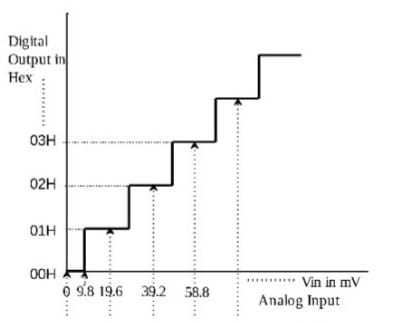
\includegraphics[width=\columnwidth]{figs/fig1.jpeg}
    \caption{Caption}
    \label{fig:ADC}
\end{figure}
\begin{enumerate}[label=(\alph*)]
    \item $64H$
    \item $65H$
    \item $66H$
    \item $67H$
\end{enumerate}

\solution
\begin{table}[!h]
    \centering
    \resizebox{\columnwidth}{!}{\begin{table}[!h]
    \centering
    \begin{tabular}{|c|c|c|}
    \hline
       \textbf{Symbol}  & \textbf{Value} &  \textbf{Description}\\
    \hline
       $V_{in}$  &  &  Input Voltage\\
    \hline
        $V_{out}$ & & Output Voltage\\
    \hline
        $f$ & $1000Hz$ & Input Wave Frequency\\
    \hline
        $T$ & $\dfrac{1}{f} = 10^{-3} s$ & Input Wave Time Period\\
    \hline
        \multirow{4}{*}{$R$} & (a) $0.5k\Omega$ & \multirow{4}{*}{Resistance}\\
        \cline{2-2}
        & (b) $5k\Omega$ &\\
        \cline{2-2}
        & (c) $0.5k\Omega$ &\\
        \cline{2-2}
        & (d) $5k\Omega$ &\\
    \hline
        \multirow{4}{*}{$C$} & (a) $0.1\mu F$ & \multirow{4}{*}{Capacitance}\\
        \cline{2-2}
        & (b) $1\mu F$ &\\
        \cline{2-2}
        & (c) $0.1\mu F$ &\\
        \cline{2-2}
        & (d) $1\mu F$ &\\
    \hline
        $\tau$ & $RC$ & Time Constant\\
    \hline
    \end{tabular}
    \caption{Given Parameters}
    \label{tab:1_gate.23.ph.37}
\end{table}
}
    \caption{Given Parameters}
    \label{tab:1}
\end{table}

Calculating the step-size:
\begin{align}
    \Delta V_{in} &= \frac{V_{max} - V_{min}}{2^n - 1}\\
    &= \frac{5 - 0}{2^8 - 1}\\
    &= \frac{5}{255}\\
   \implies V_{out} &= \frac{V_{in}}{\Delta V_{in}}\\
    &= \frac{1.9922 \times 255}{5}\\
    &= 101.59\\
    &\approx 102_{10}\\
    &= (66)_{H}
\end{align}

$\therefore$ correct answer is option (c).
\end{document}
